\section{Generic Crypto Interface}


\begin{frame}

\frametitle{Contexts}

\underline{Algorithms which need configurations}
\begin{itemize}
  \item \footnotesize{Hash}
  \item \footnotesize{Signature}
  \item \footnotesize{Symmetric cipher}
  \item \footnotesize{Asymmetric cipher}
  \item \footnotesize{Diffie-Hellman}
\end{itemize}

\vspace{0.25cm}

\underline{Contexts}:
\begin{itemize}
  \item \footnotesize{Represent state of stateful algorithms}
  \item \footnotesize{No hidden states in the interface}
\end{itemize}

\end{frame}


\begin{frame}

\frametitle{Context example: Hash}


% trim: left, bottom, right, up
\centering
{
\only<1>{

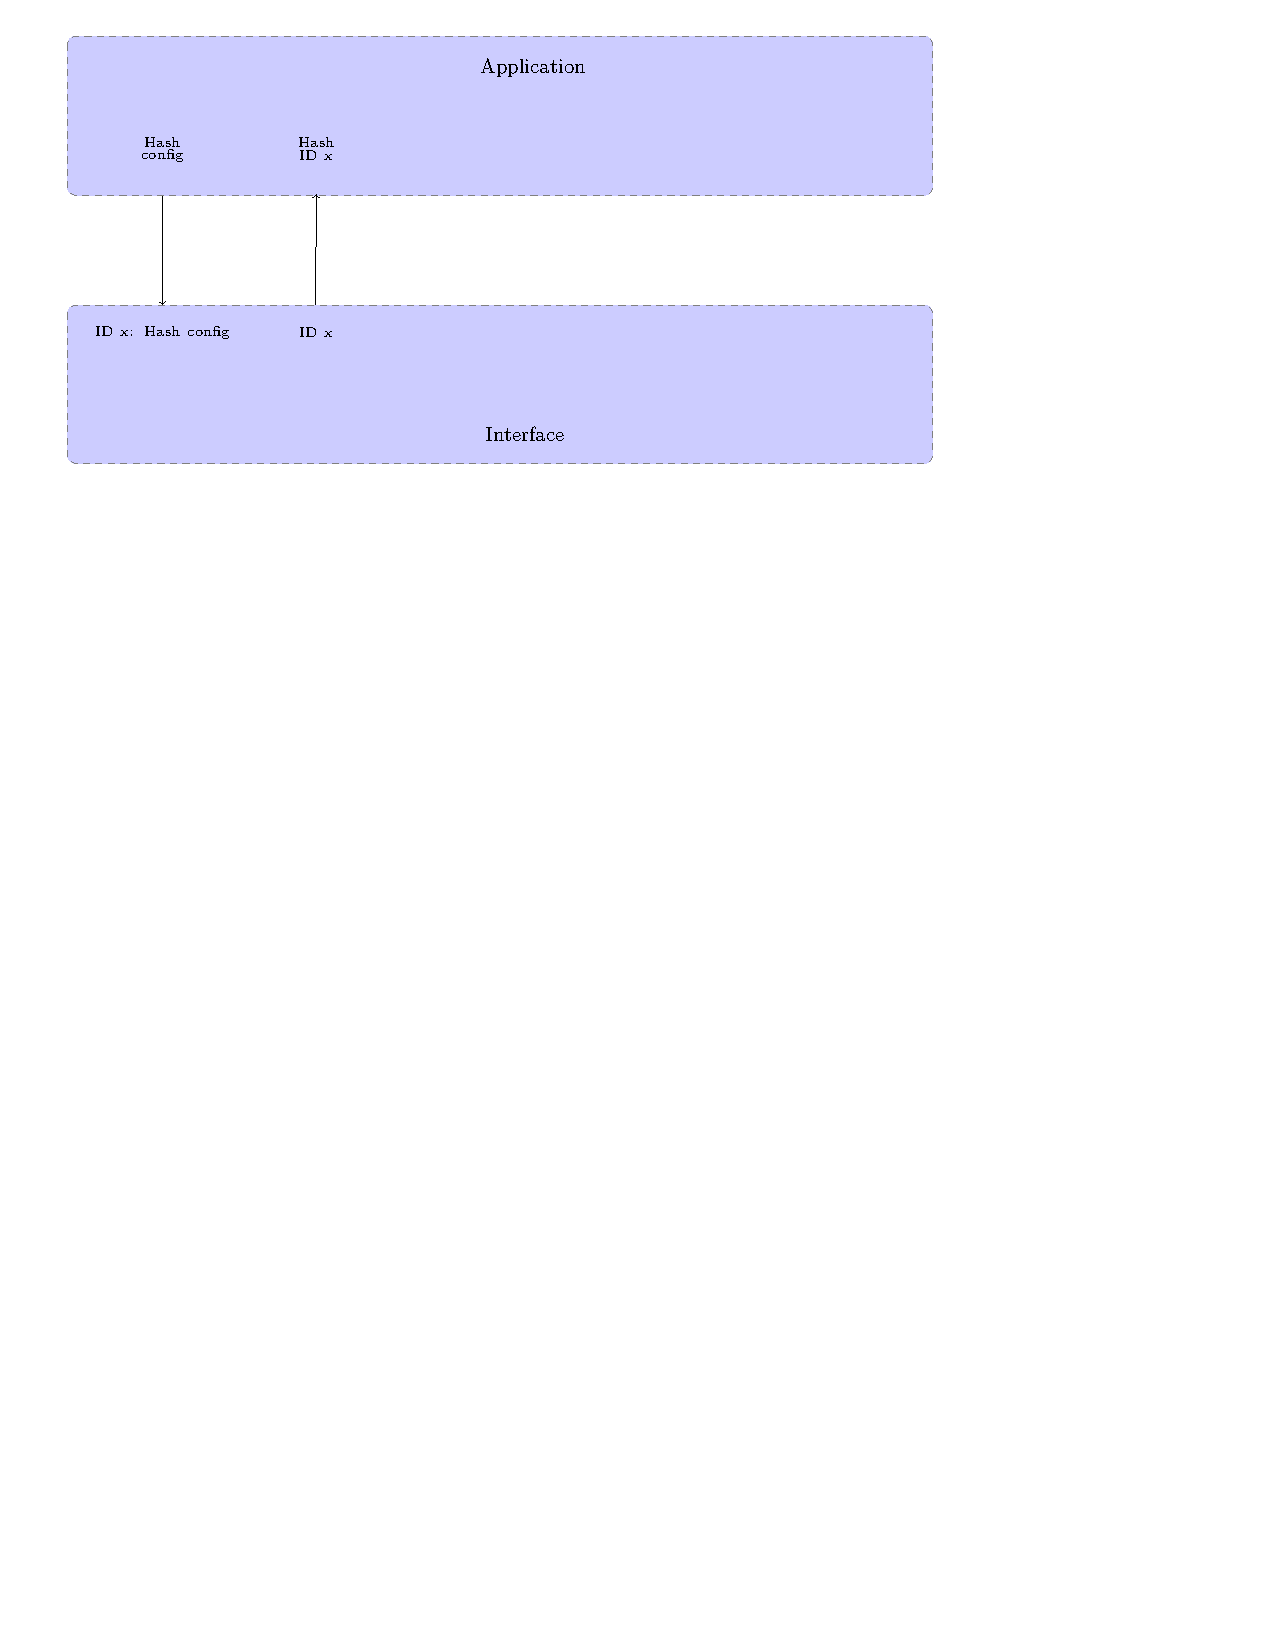
\includegraphics[trim=2cm 20cm 7cm 0cm,
height=5cm]{figures/interface_hash_example_config.pdf} 

}


\only<2>{

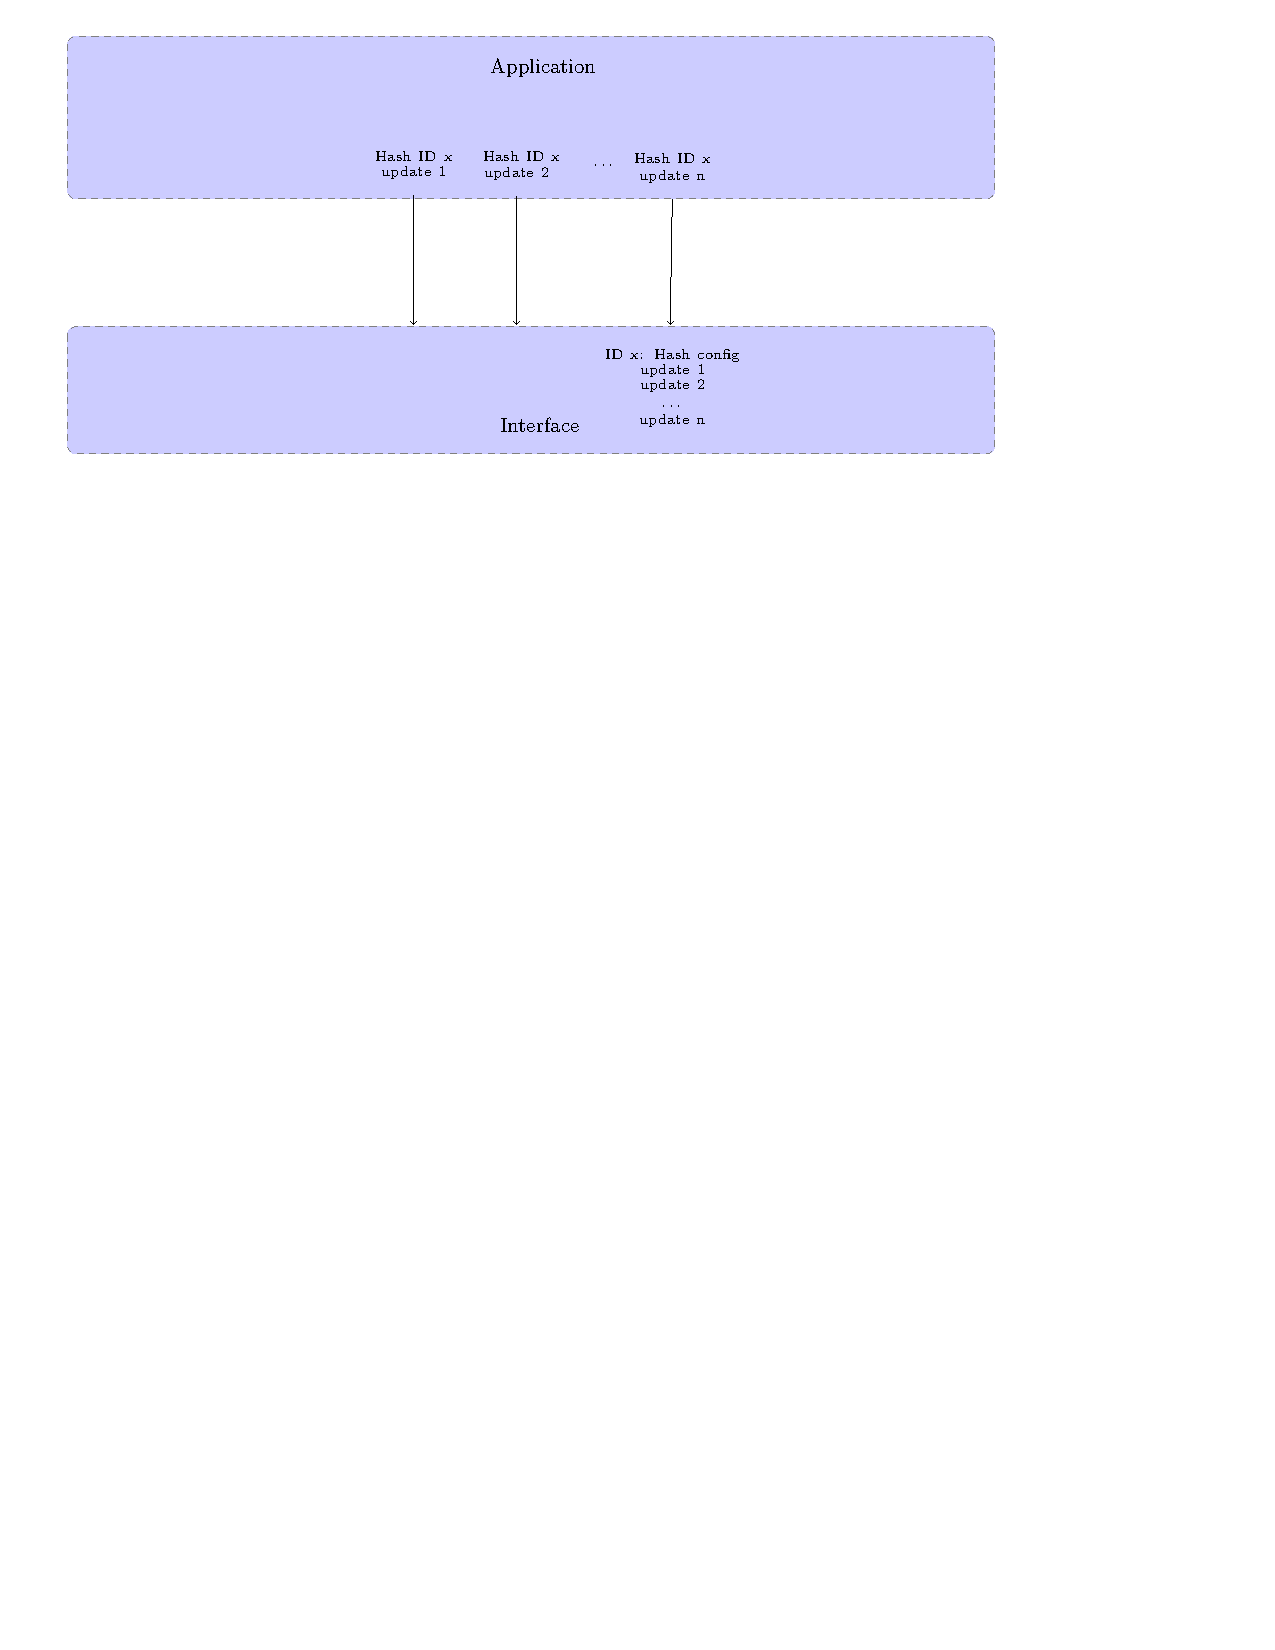
\includegraphics[trim=2cm 20cm 7cm 0cm,
height=5cm]{figures/interface_hash_example_update.pdf} 

}


\only<3>{

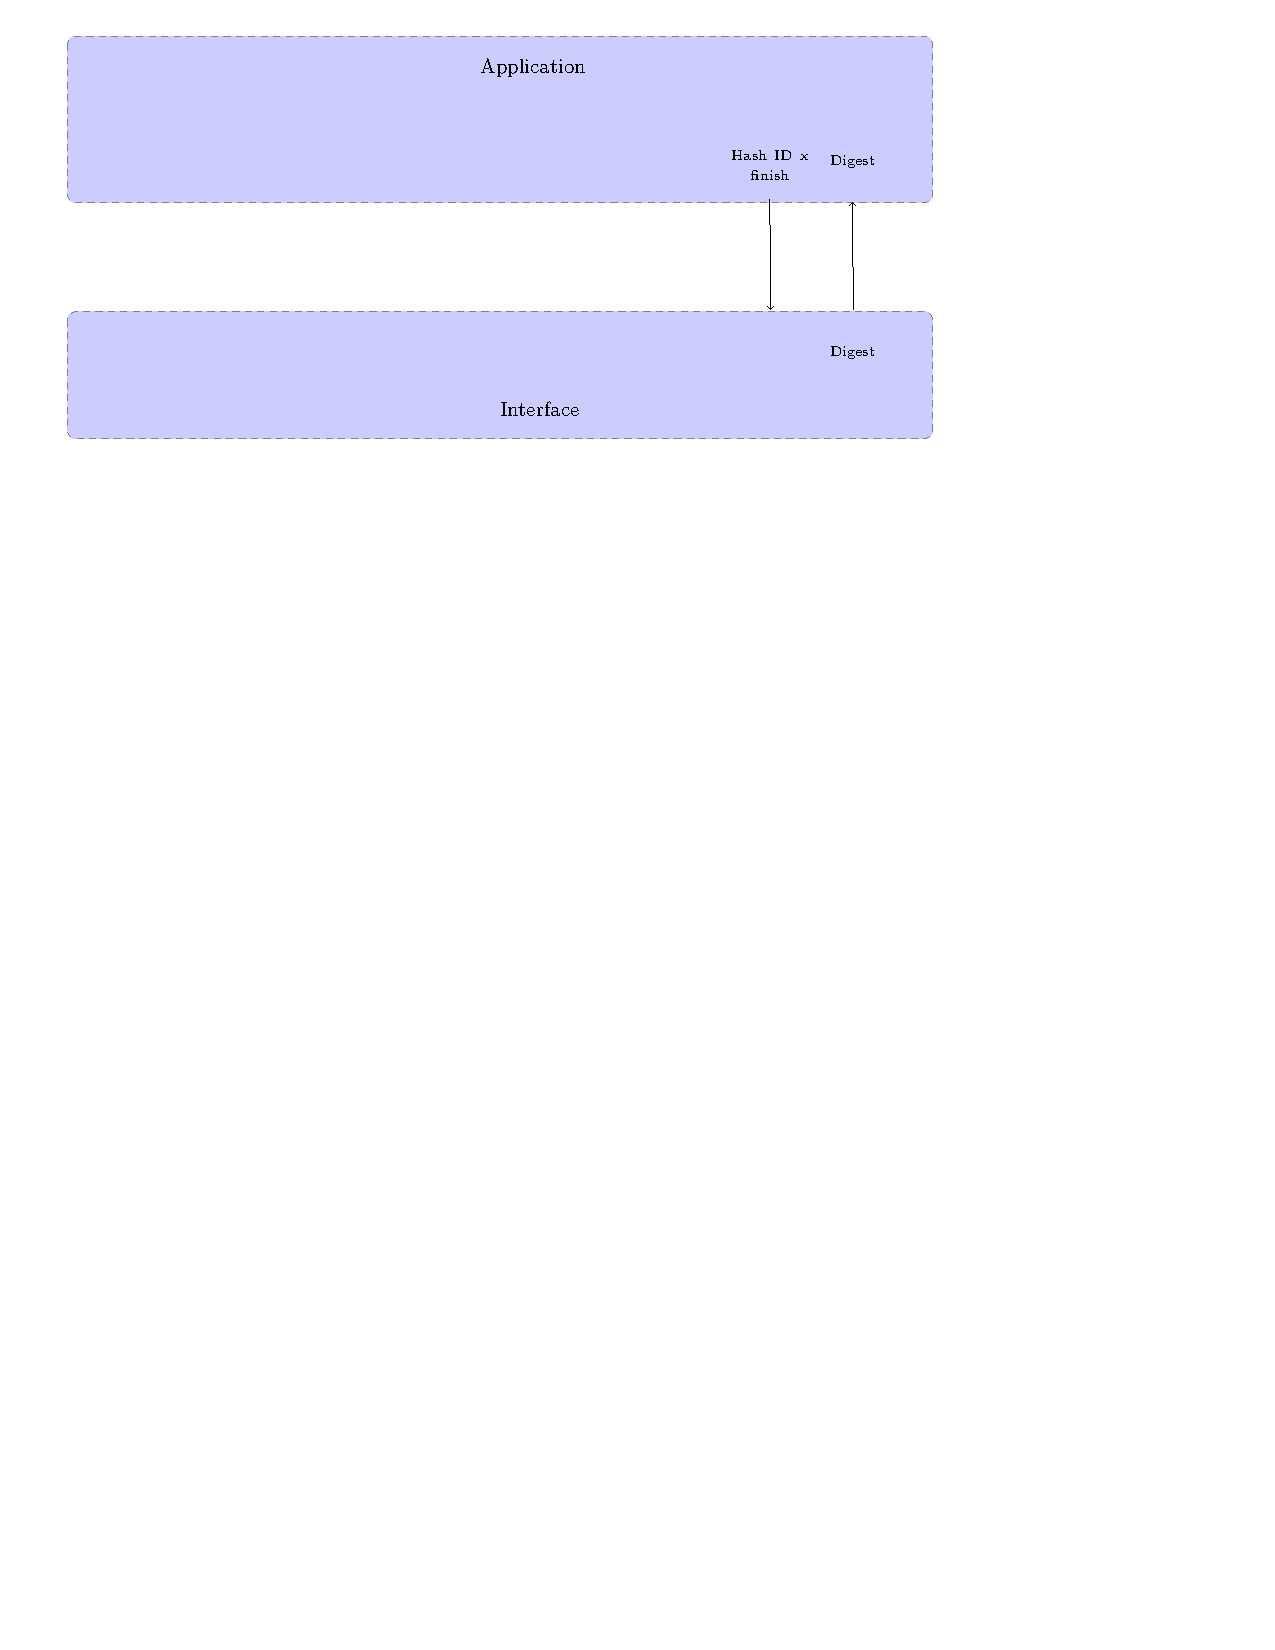
\includegraphics[trim=2cm 20cm 7cm 0cm,
height=5cm]{figures/interface_hash_example_finish.pdf} 

}

}


\begin{enumerate}
  \item \footnotesize{Create the hash context with the desired configuration}
  \pause
  \item \footnotesize{Update the hash context by adding messages}
  \pause
  \item \footnotesize{Get the digest}
\end{enumerate}


\end{frame}


\begin{frame}

\frametitle{Context Hash/Signature: Clone}

\begin{columns}



\begin{column}{0.4\textwidth}

%\frame{
% trim: left, bottom, right, up
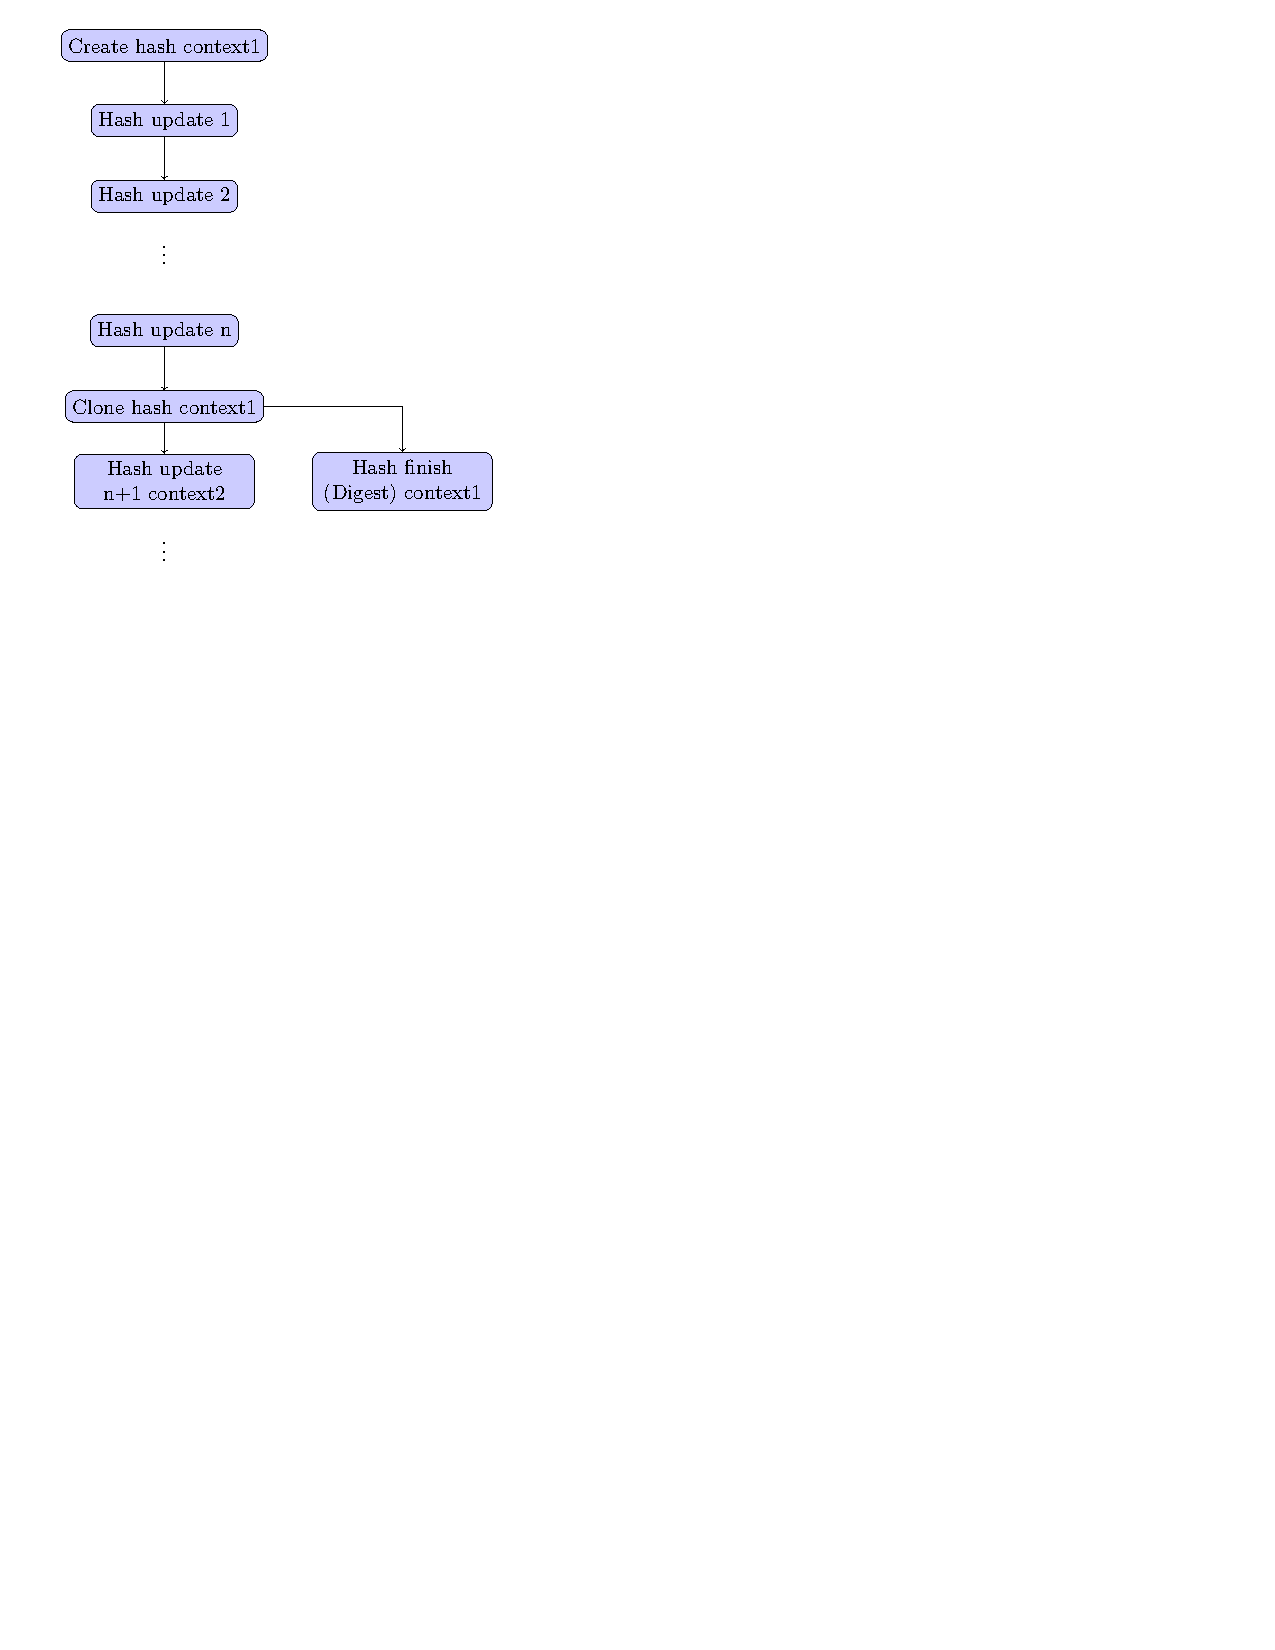
\includegraphics[trim=1cm 17cm 13cm 0cm,
height=7cm]{figures/hash_signature_clone.pdf} 
%}

\end{column}

\begin{column}{0.5\textwidth}


\underline{Problems}:
\begin{itemize}
  \item \footnotesize{Once the digest has been computed no more updates could be done}
  \item \footnotesize{Only the release of the context is possible}
\end{itemize}

\vspace{0.25cm}

\underline{Solution}: Clone of the context
\begin{itemize}
  \item \footnotesize{Copy of the configuration and the updates of the actual context
  in another context}
  \item \footnotesize{Digest can be calculated for one context}
  \item \footnotesize{Other messages can be added to the other context}
\end{itemize}


\end{column}

\end{columns}

\end{frame}